\documentclass[12pt,a4paper]{report}

%adjust your page margins here
\usepackage[top=0.70in, bottom=0.70in, left=0.8in,right=0.80in]{geometry} % setting the page alignment with this package
\usepackage[pdftex]{graphicx} %for embedding images
\usepackage[%dvips, % commented for pdflatex
bookmarks,  colorlinks=false]{hyperref} %for creating links in the pdf version and other additional pdf attributes, no effect on the printed document
\hypersetup{%
    pdfborder = {0 0 0}
}
\usepackage[final]{pdfpages} %for embedding another pdf, remove if not required
\usepackage{float} %used for figure placement with H as a parameter

\usepackage{hyperref}
\hypersetup{
    colorlinks=true,
    linkcolor=blue,
    filecolor=magenta,      
    urlcolor=cyan,
}
 
\urlstyle{same}
\usepackage{pslatex} % for times new roman, old package, but works
\usepackage{array} % for making text bold in table
\usepackage{setspace}
\usepackage{float}
\usepackage{enumerate}
\usepackage{longtable}

\usepackage[font=small,labelfont=bf]{caption}
\def\figurename{\textbf{Figure }}

\usepackage{listings}
\usepackage{color}

\definecolor{dkgreen}{rgb}{0,0.6,0}
\definecolor{gray}{rgb}{0.5,0.5,0.5}
\definecolor{mauve}{rgb}{0.58,0,0.82}
 
\lstset{ %
  language=Java,                % the language of the code
  basicstyle=\footnotesize,           % the size of the fonts that are used for the code
  numbers=left,                   % where to put the line-numbers
  numberstyle=\tiny\color{gray},  % the style that is used for the line-numbers
  stepnumber=1,                   % each line is numbered
  numbersep=5pt,                  % how far the line-numbers are from the code
  backgroundcolor=\color{white},      % choose the background color. You must add \usepackage{color}
  showspaces=false,               % show spaces adding particular underscores
  showstringspaces=false,         % underline spaces within strings
  showtabs=false,                 % show tabs within strings adding particular underscores
  frame=single,                   % adds a frame around the code
  rulecolor=\color{black},        % if not set, the frame-color may be changed on line-breaks within not-black text (e.g. commens (green here))
  tabsize=2,                      % sets default tabsize to 2 spaces
  captionpos=b,                   % sets the caption-position to bottom
  breaklines=true,                % sets automatic line breaking
  breakatwhitespace=false,        % sets if automatic breaks should only happen at whitespace
  title=\lstname,                   % show the filename of files included with \lstinputlisting;
                                  % also try caption instead of title
  keywordstyle=\color{blue},          % keyword style
  commentstyle=\color{dkgreen},       % comment style
  stringstyle=\color{mauve},         % string literal style
  escapeinside={\%*}{*)},            % if you want to add a comment within your code
  morekeywords={*,...}               % if you want to add more keywords to the set
}

%For the header and footer
\usepackage{fancyhdr}
\fancypagestyle{plain}{%
\fancyfoot[L]{\emph{RUBE GOLDBERG Physics Simulation,CS251 Project, IIT Bombay}} % except the center
\fancyfoot[R]{\thepage}
\renewcommand{\headrulewidth}{0.4pt}
\renewcommand{\footrulewidth}{0.4pt}
}

\pagestyle{fancy}

\rhead{\emph{Bucket Alarm}}

\fancyfoot[LO,LE]{\emph{RUBE GOLDBERG Physics Simulation,CS251 Project, IIT Bombay}}
\cfoot{}
\fancyfoot[RO, RE]{\thepage}
\renewcommand{\headrulewidth}{0.4pt}
\renewcommand{\footrulewidth}{0.4pt}
%For the header and footer Over

%Page Border
\usepackage{pgf}
\usepackage{pgfpages}

\pgfpagesdeclarelayout{boxed}
{
  \edef\pgfpageoptionborder{0pt}
}
{
  \pgfpagesphysicalpageoptions
  {%
    logical pages=1,%
  }
  \pgfpageslogicalpageoptions{1}
  {
    border code=\pgfsetlinewidth{2pt}\pgfstroke,%
    border shrink=\pgfpageoptionborder,%
    resized width=.95\pgfphysicalwidth,%
    resized height=.95\pgfphysicalheight,%
    center=\pgfpoint{.5\pgfphysicalwidth}{.5\pgfphysicalheight}%
  }%
}
\pgfpagesuselayout{boxed}
\setlength{\parindent}{1cm}
%GLOBAL SETTINGS OVER, DOCUMENT BEGINS
\begin{document}
\renewcommand\bibname{References}
\lhead{ }

%FROM HERE YOUR PAGES START GETTING ADDED

% includes the cover page
\newpage
\begin{center}
\thispagestyle{empty}
\Large{\textbf{PROJECT REPORT\\ \large{FOR}}}\\[0.7cm]
\LARGE{\textsc {\textbf{LAB09}}}\\[0.5cm]
\vspace{0.5cm}
\Large{\textbf{\\Submitted to}}
\LARGE{\textbf{\\CS251\\IIT BOMBAY\\}}
\vspace{1cm}
\Large{\textbf{\\A report on Box2d simualation\\with GPROF\\}}
%\Large{\textbf{\\BACHELOR'S DEGREE IN\\COMPUTER ENGINEERING}}
\vspace{1cm}
\Large{\textbf{\\BY}}\\[0.5cm]
\begin{table}[h]
\centering
\Large{
\begin{tabular}{>{\bfseries}lc>{\bfseries}r}
Vishal Babu Bhavani & & 140050049\\Pushyarag Yadagiri & & 140050047\\Divakar Reddy Naru & & 140050044\\
\end{tabular}}
\end{table}
\vspace{0.5cm}
\large{\textbf{Under the Mentorship and Guidance of}}\\
\large{\textbf{Prof. Sharat Chandran\\ IIT Bombay}}\\
\vspace{1cm}
%\large{\textbf{DEPARTMENT OF COMPUTER ENGINEERING}}\\
%\Large{\textbf{NAME OF COLLEGE}}\\
%\large{\textbf{LOCATION IN PUNE, PUNE - PINCODE}}
%\large{\textbf{\\2012-2013}}\\
%\vspace{1cm}

\Large{\textbf{AFFILIATED TO\\}}
\LARGE{\textbf{CS251 LAB}}\\
\vspace{1cm}
\large{\textbf{October 2015}}\\
\vspace{1cm}
\newpage
\end{center}
\newpage

%\newpage
\begin{center}
\thispagestyle{empty}
\Large{\textbf{A PROJECT REPORT\\ON}}\\[0.3cm]
\Large{\textsc {\textbf{``NAME OF PROJECT''}}}\\
\Large{\textbf{\\Submitted to}}
\LARGE{\textbf{\\UNIVERSITY OF PUNE\\}}
\large{\textbf{\\In Partial Fulfilment of the Requirement for the Award of\\}}
\LARGE{\textbf{\\BACHELOR'S DEGREE IN\\COMPUTER ENGINEERING}}
\vspace{0.3cm}
\Large{\textbf{\\BY}}\\[0.3cm]
\begin{table}[h]
\centering
\Large{
\begin{tabular}{>{\bfseries}lc>{\bfseries}r}
GROUP MEMBER A & & ROLL NUMBER A\\GROUP MEMBER B & & ROLL NUMBER B\\GROUP MEMBER C & & ROLL NUMBER C\\GROUP MEMBER D & & ROLL NUMBER D\\
\end{tabular}}
\end{table}
\large{\textbf{UNDER THE GUIDANCE OF}}\\
\large{\textbf{PROF. GUIDE NAME}}\\[0.5cm]
\includegraphics[scale=0.5]{project/images/jscoe_logo}\\
\large{\textbf{DEPARTMENT OF COMPUTER ENGINEERING}}\\
\Large{\textbf{NAME OF COLLEGE}}\\
\large{\textbf{LOCATION IN PUNE, PUNE - PINCODE}}
\large{\textbf{\\2012-2013}}\\[0.5cm]
\Large{\textbf{AFFILIATED TO}}\\[0.5cm]
\includegraphics[scale=5.0]{project/images/uop-logo}\\
\LARGE{\textbf{UNIVERSITY OF PUNE}}
\newpage

\end{center}
%\newpage

% includes the certificate page
%\input{project/certificate.tex} 
%\newpage

% includes the acknowledgements page
\begin{center}
\thispagestyle{empty}
\LARGE{\textbf{Acknowledgements}}\\[1cm]
\end{center}
\linespread{1.13}
\large{\paragraph{}We are profoundly grateful to \textbf{Professor Sharat Chandran} for the expert guidance
and continuous encouragement throughout to see that this project rights its
target since its commencement to its completion.}
\large{\paragraph{}We must express our sincere heartfelt gratitude to all the TA's who helped us directly or indirectly during this course of work
we are also very grateful to many of the online tutorials like \cite{Tizen}, \cite{Box2DforFlashGames}, \cite{Box2Dlinks}, \cite{Sharelatexlinks}, \cite{csslinks}
and \cite{Bessierlinks}.
}

\begin{flushright}
{
Vishal Babu Bhavani\\
Pushyarag Yadagiri\\
Divakar Reddy Naru\\

}
\end{flushright}
\newpage
 
\newpage

%\input{project/abstract.tex} % adds the Research Methodology page
\newpage

%TABLE OF CONTENTS AND LIST OF FIGURES ARE AUTOMATICALLY ADDED BY FOLLOWING COMMANDS
%ADD FIGURE OF TABLES IF YOU NEED TO, CHECK DOCUMENTATION
\pagenumbering{roman} %numbering before main content starts


%To reset the Header & Footer for TOC and LOF
\pagestyle{empty}
\addtocontents{toc}{\protect\thispagestyle{empty}}
\tableofcontents % adds Index Page

\addtocontents{lof}{\protect\thispagestyle{empty}}
\listoffigures % adds List of Figures
\cleardoublepage

%And reset back the settings we choose for Header and Footer
\pagestyle{fancy}

\newpage
\pagenumbering{arabic} %reset numbering to normal for the main content

\chapter{Introduction}
\section{RUBE GOLDBERG MACHINE}
\subsection{About Rube Goldberg machine}
\paragraph{}
This report is made to describe the concepts behind our CS251
project Box2d simulation.
 In this project we have created a simulation of a Rube Goldberg machine we designed, in C++ using the Box2D library.
 A Rube Goldberg machine is a contraption that performs a simple task in a complicated fashion.
 We have created a GUI interface for visualization of the simulation and a non-GUI version for analysis of code statistics. We profile the code using gprof, the inbuilt Linux profiling tool, in order to identify which part of the simulation is taking the maximum amount of time to execute. Using this information, we optimize the code. In this report we have given a gist of our design, its salient features and working. Also this report gives the observations on the profiling of the code and the possible optimizations that can be done.
 
 
 

\subsection{About our project}
\paragraph{}

Our main motive of doing this project is to get to know and work with a lot off new stuff like box2d, makefiles,etc and learn the application of all the things we learned in this course.

The project is about a bucket alarm which will pour water on a sleeping person.
Our main idea is to keep the clock going,and make arrangements such that the contraption starts and finally invert the bucket of water so that the water falls on the person so he wakes up.

 % adds the introduction page
%\input{project/literature-survey.tex} % adds the Literature Survey page
\chapter{Software Requirements Specification}
\section{SPECIFIC REQUIREMENT}
\subsection{Overall Description}
\paragraph{This project is made using Box2D ,an open source 2D physics engine for games.The whole project is coded in C++.
The  User Interface is easy to handle.User needs to set the alarm in the clock by clicking on the clock.This section uses the mouse click feature of Box2d to set the timeSo the user should make sure that the MATLAB software he/she is running must be up to date.The project is built in Box2d 2.3.0  version and developed on Ubuntu Operating System. }
\subsection{External Interface Requirement}
\paragraph{
The UI is the testbed,which is a unit-testing framework and demo environmentThe testbed is written using freeglut and GLUI.}
\begin{itemize}
 \item{
freeglut and GLUI must be pre-installed.}
 \item{keyboard and mouse are required for giving input using the interface(testbed).}
 \item{Moniter is required for output.}
 \end{itemize}


\subsection{Functional Requirement}
\begin{itemize}
 \item{Supported on Ubuntu Operating System}
 \item{g++ compiler is required as it is required for compiling the project.
the compiler must support new features included in c++11}
 \item{make and cmake utilities must be preinstalled for proper compiling of source files.
}
\end{itemize}
\chapter{Implementation}
\paragraph{}The following is implementation and detailed description of different parts of the simulation

\section{Seesaw}
\paragraph{
The see saw is made using a rectangular box and a triangle
the Box is a object of Dynamic type whreas the triangle is of static type.
both are connected using a revolute joint \textbf{LINK}.which allows free rotation of the box about the vertex of the triangular base.
Initially a square block rests on the left arm of the seesaw.
the ball from top falls on right arm of the seesaw which projects the square block into the air.
}
\begin{figure}[H]
  \centering
    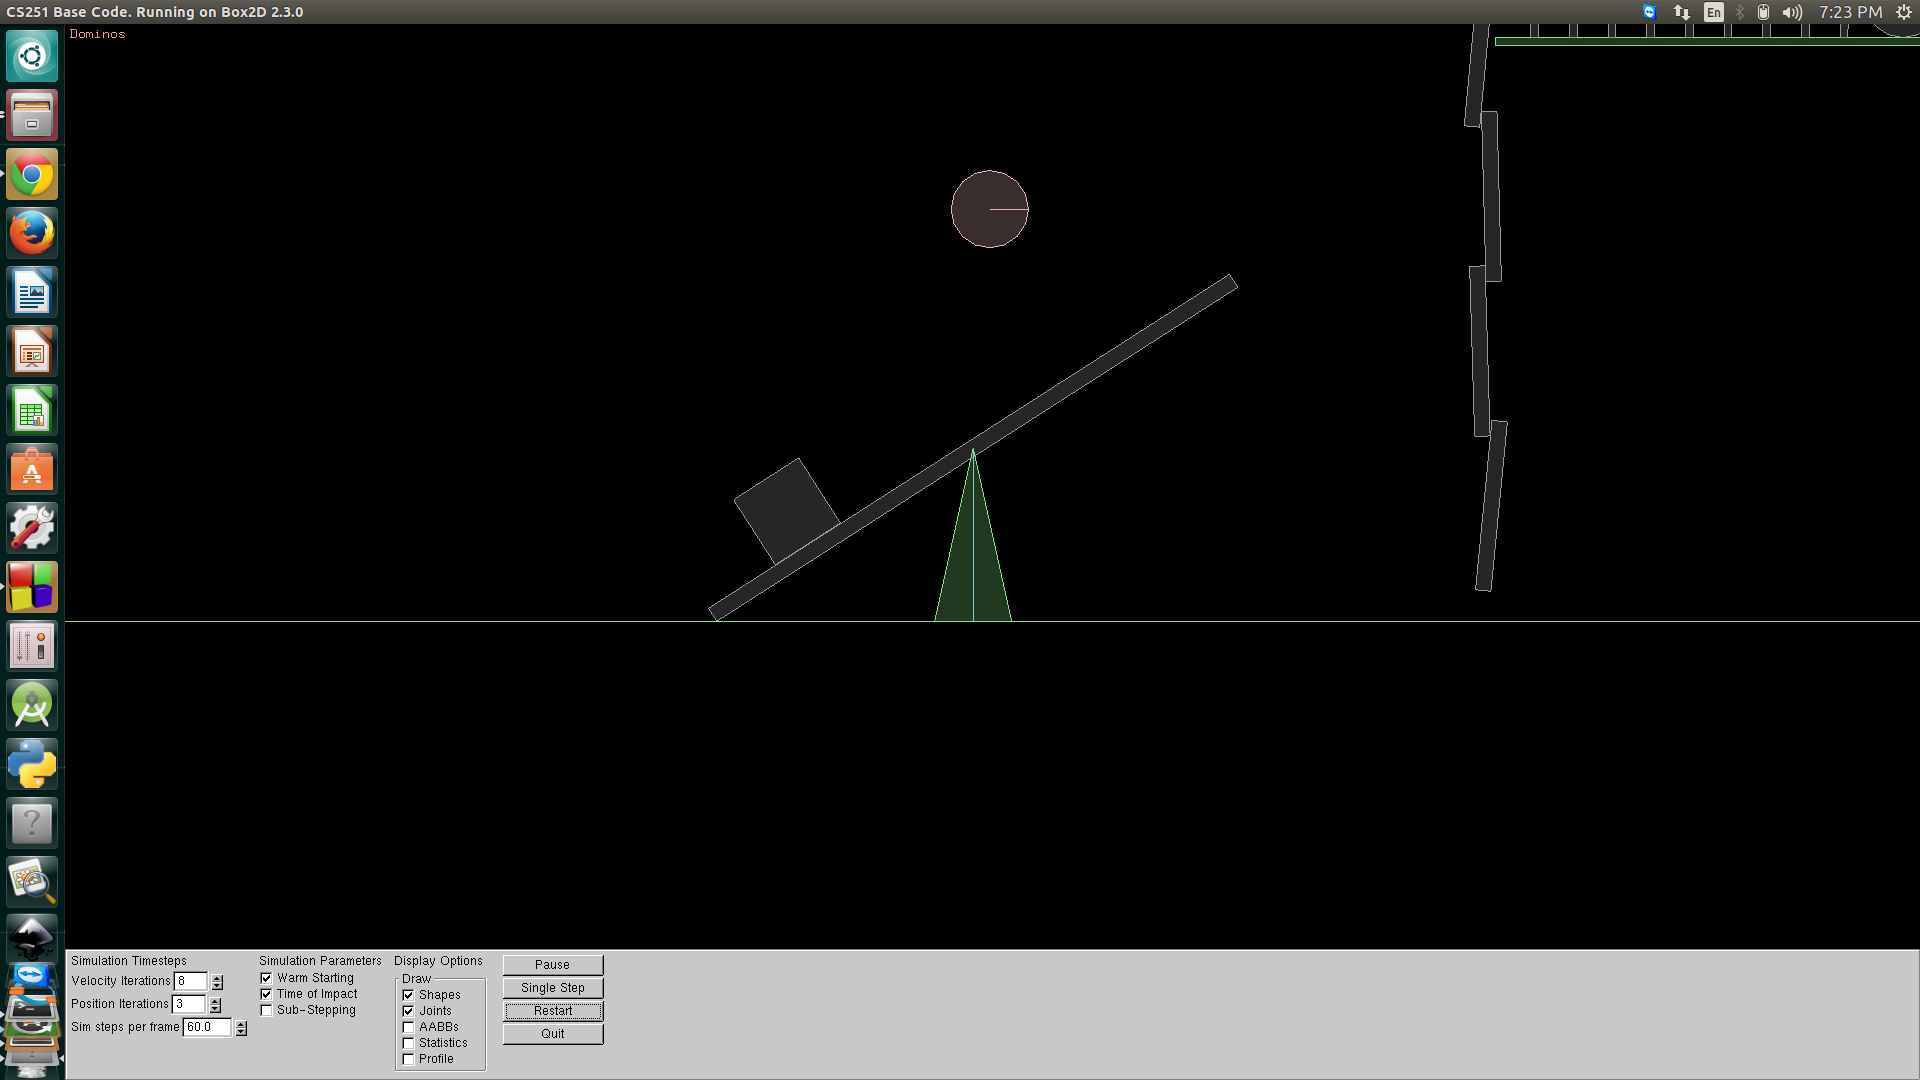
\includegraphics[scale=0.2]{project/images/pulley.png}
  \caption{\textbf{SEESAW}}
\end{figure}

\section{Pulley1}
\paragraph{
This pulley is made using an open box and a long rectangular box which are connected using the pulley joint\textbf{LINK},which makes one body move up when the other moves down and vice-versa.
Initially the pulley is balanced ie.,weights of open box and the long planc are balanced.
now the square block which flew from the left arm of the seesaw falls in the open box connected to the left arm of the pulley.
the pulley gets unbalancedand hence the open box starts going down and the plank on the right side starts to rise.
It then collides with a rotatable planc on which a ball is resting
}
\begin{figure}[H]
  \centering
    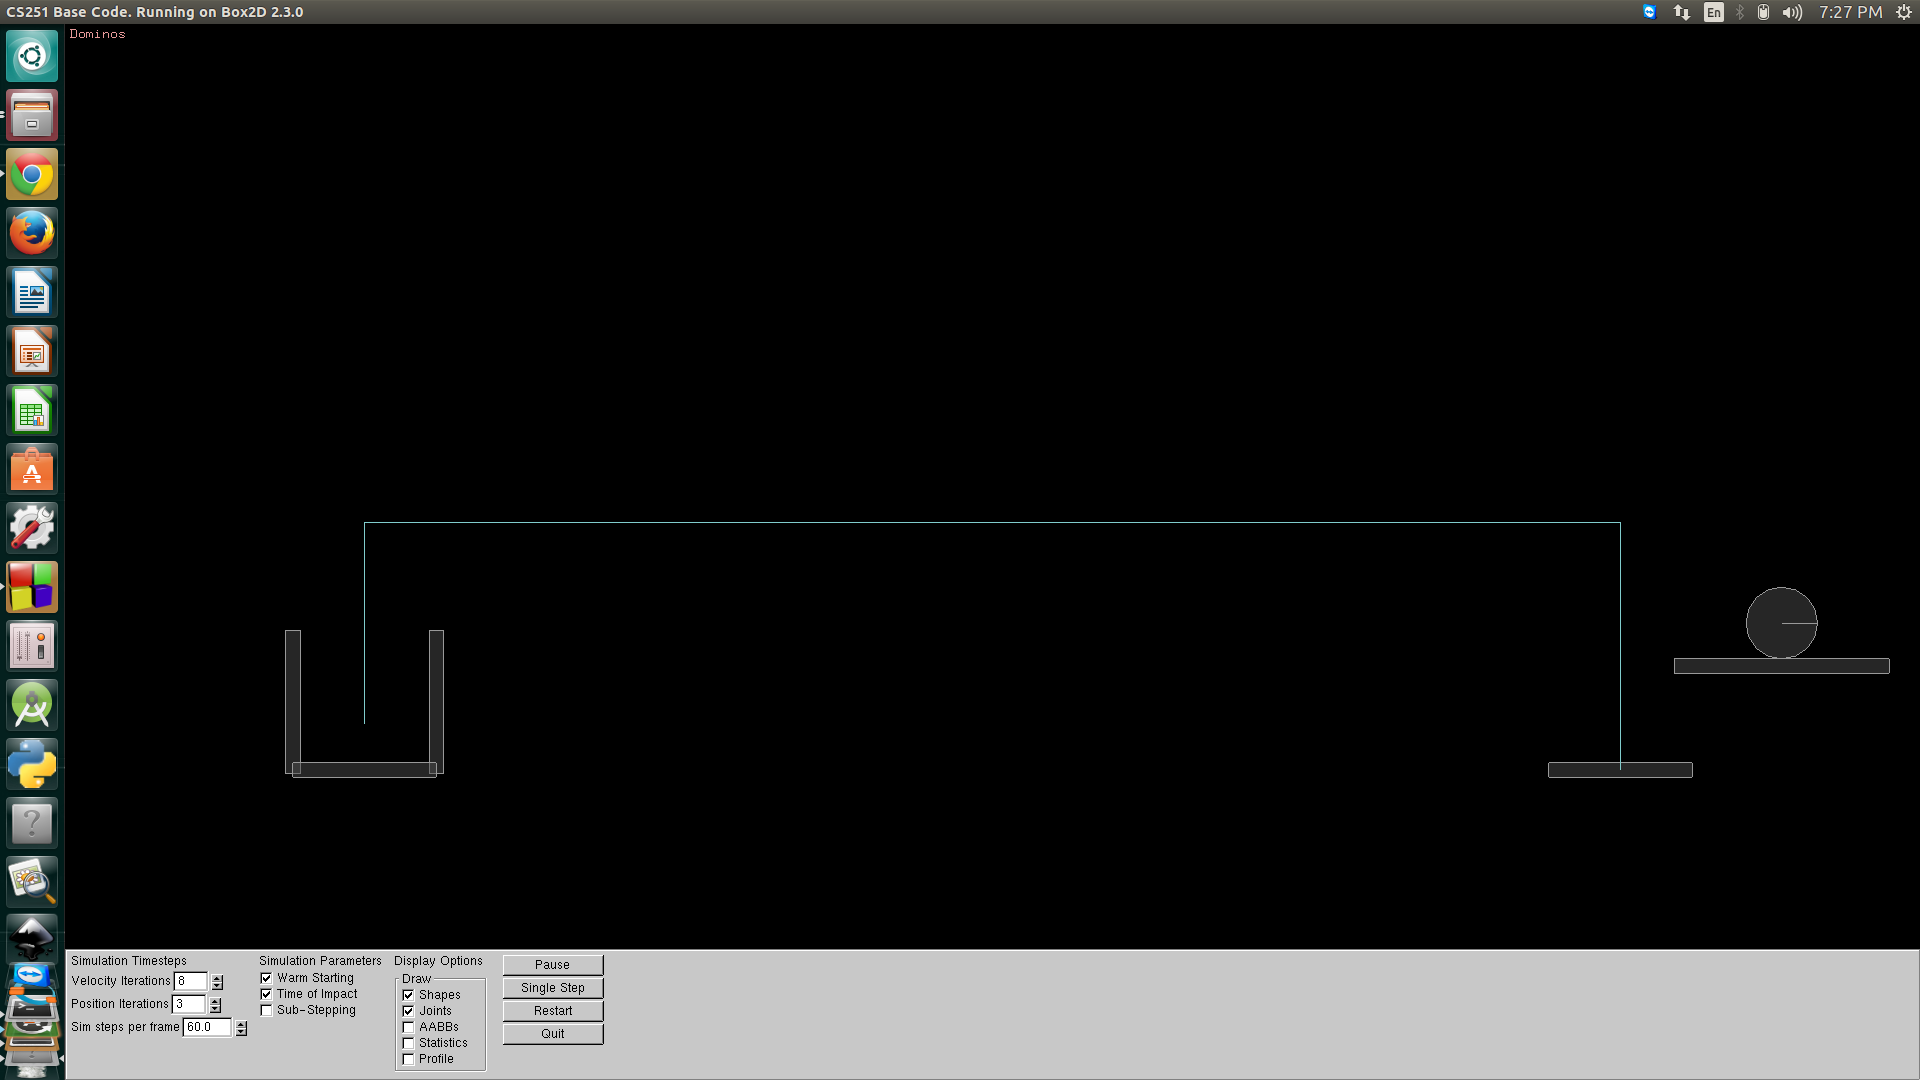
\includegraphics[scale=0.2]{project/images/pulley2.png}
  \caption{\textbf{PULLEY}}
\end{figure}


\section{the set of rotatable plancks}
\paragraph{
These are made using a rectangular block and a small static box used as the hinge at the ceter which are connected using the revolute joint\textbf{LINK},which makes the planck free to rotate about it's center.
Meanwhile the first ball which fell on the left arm of the seesaw falls of the seesaw and goes right and hits the lowest plank.
which triggers a series of collisions between the rotatable planks.
the top most plank now collides with the dominoes.
the dominoes now get triggered and the fall one by one and finally they collide with a ball which starts moving right.
}
\begin{figure}[H]
  \centering
    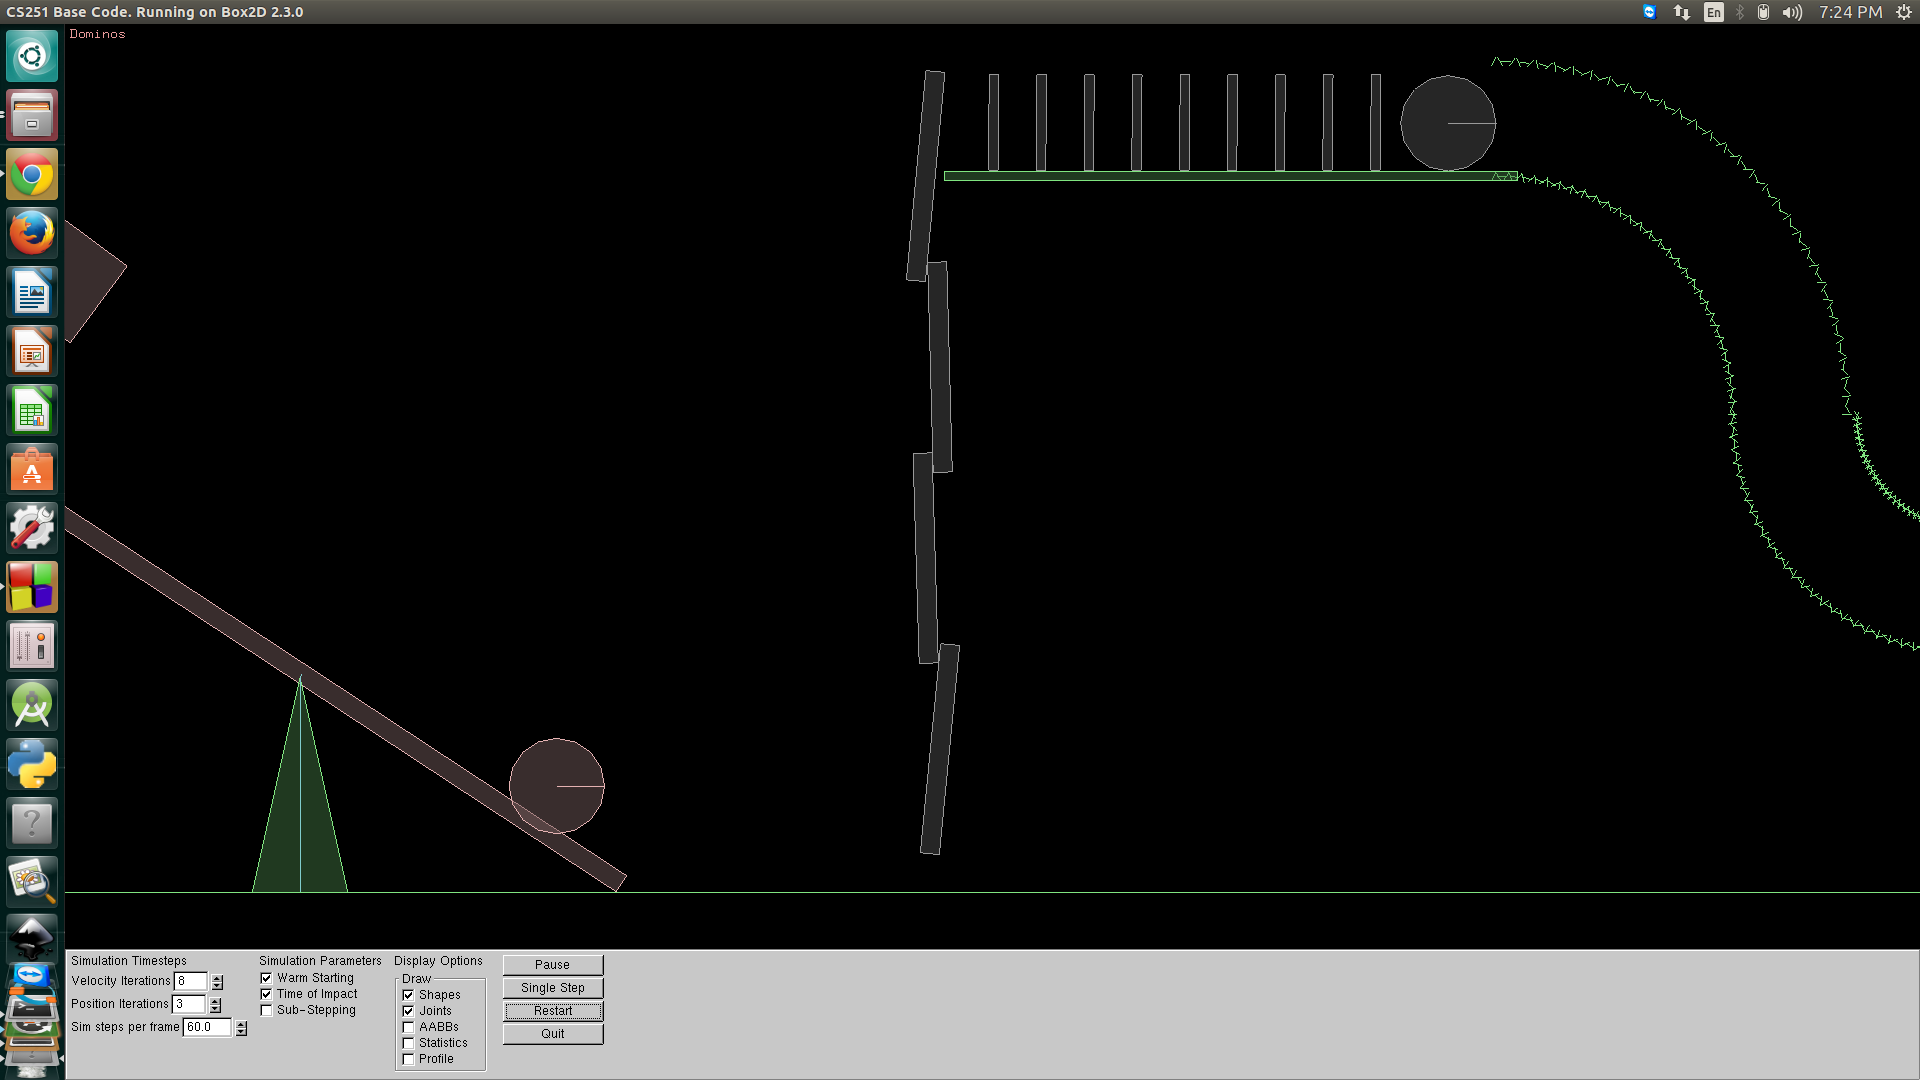
\includegraphics[scale=0.2]{project/images/plating.png}
  \caption{\textbf{ROTATABLE PLANES}}
\end{figure}

\section{the second set of rotatable plancks}
\paragraph{
These are made using a rectangular block and a small static box used as the hinge at the ceter which are connected using the revolute joint\textbf{LINK},which makes the planck free to rotate about it's center.
Meanwhile the floating  ball which                                moves up and hits the leftmost plank,which triggers a series of collisions between the rotatable planks each of which is supporting a ball.each plank rotates and triggers the next plank to rotate by colliding.now all the planks rotate and all the balls on them fall on the static ramp below them.
}
\begin{figure}[H]
  \centering
    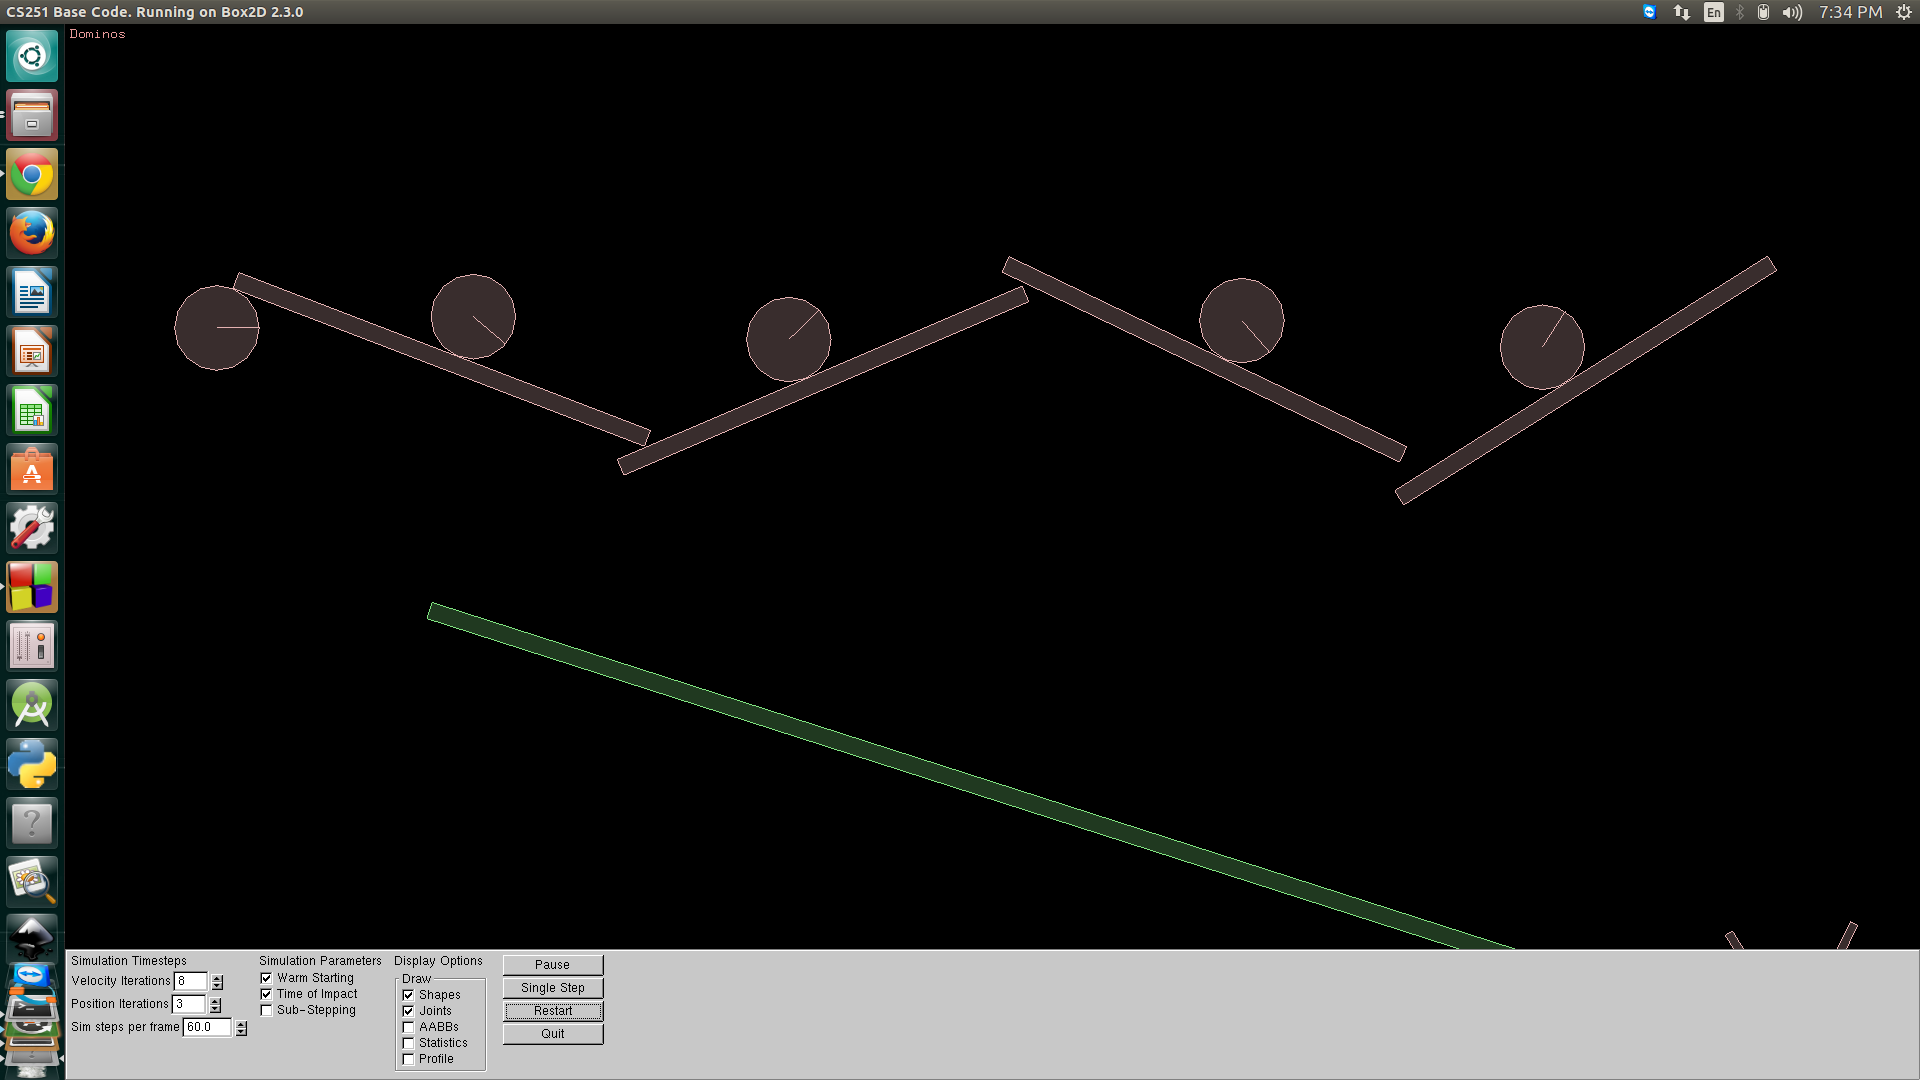
\includegraphics[scale=0.2]{project/images/revolvers.png}
  \caption{\textbf{SECOND SET OF ROTATING PLANES}}
\end{figure}

\section{The motor}
\paragraph{
These are made using 3 thin rectangular blocks and a small static box used as the hinge at the ceter which are connected using the revolute joint\textbf{LINK},which makes the plancs free to rotate about it's center.also the motor feature of the revolute joint is enabled so that it rotates at a particular speed.
Meanwhile the  balls come rolling on the ramp fall on the motor.
The motor sends the balls one by one into the open box of the second pulley.
}
\begin{figure}[H]
  \centering
    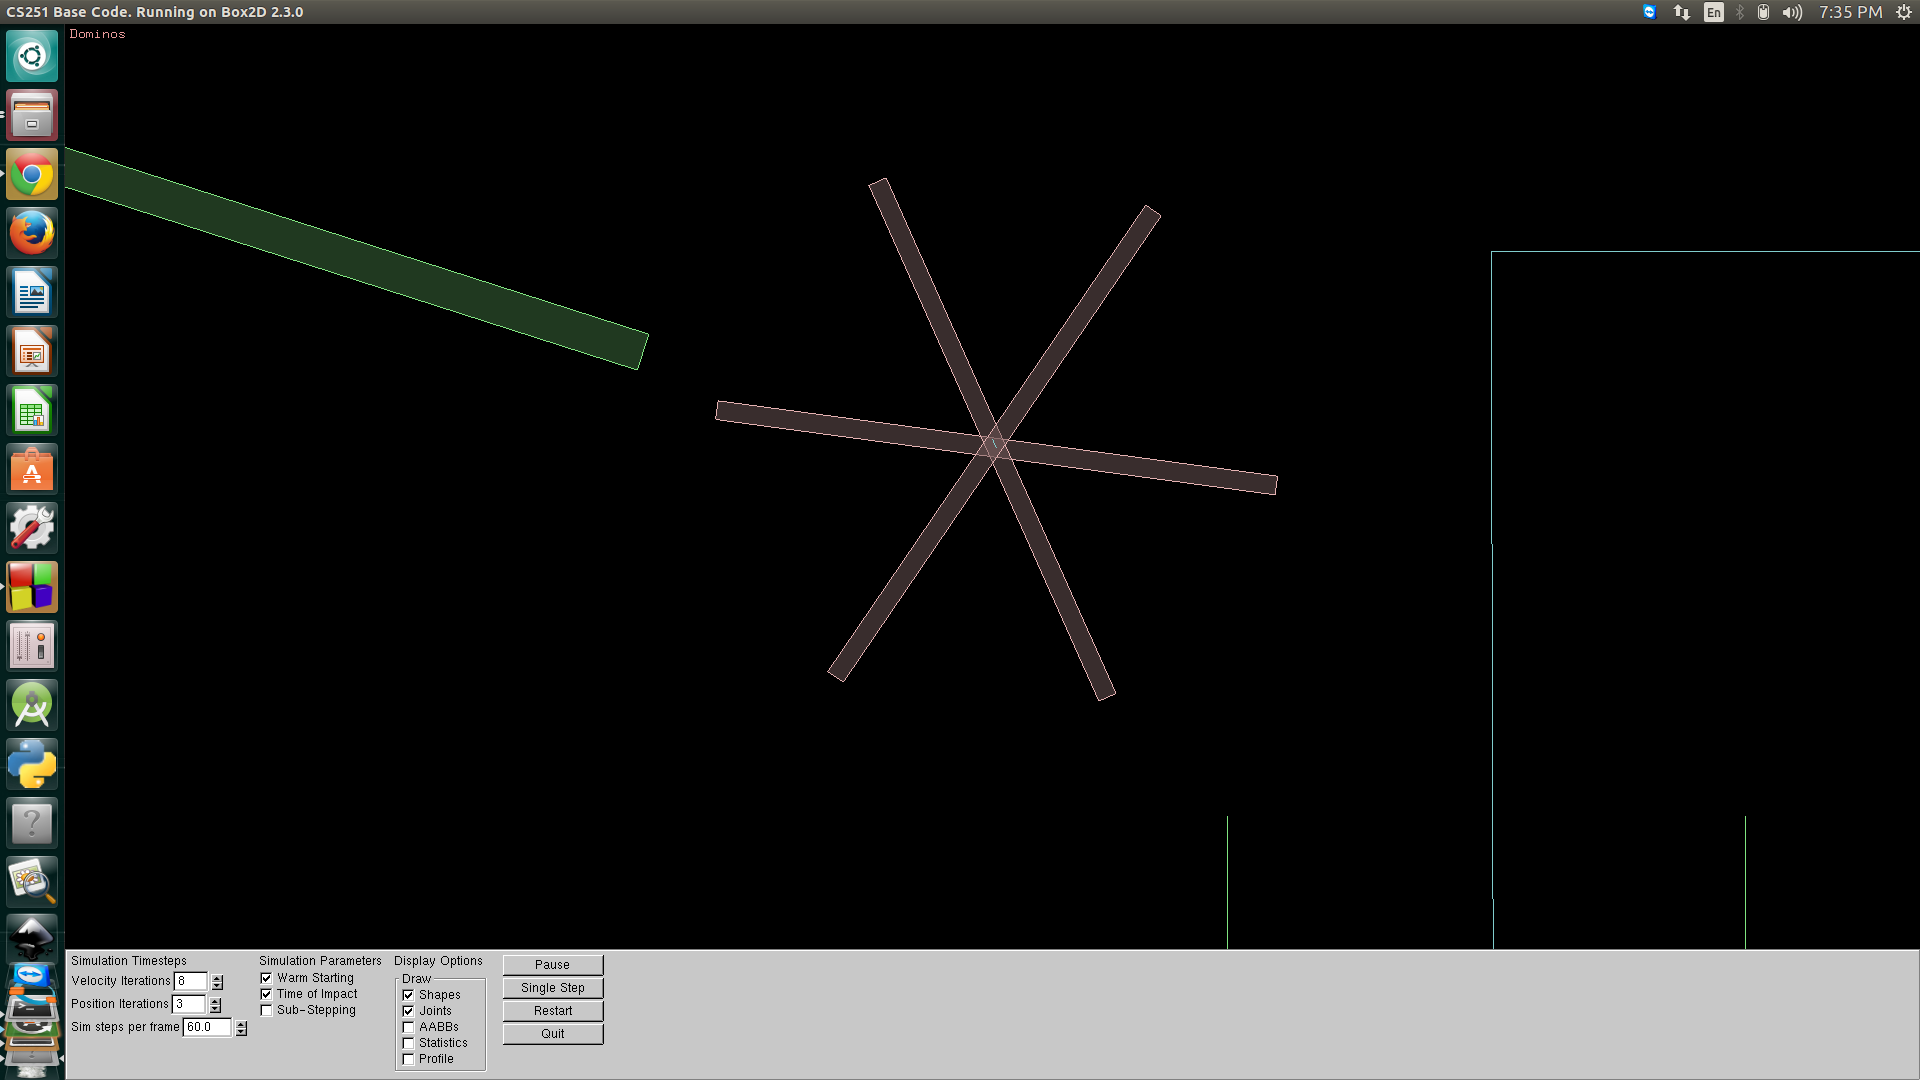
\includegraphics[scale=0.2]{project/images/rotor.png}
  \caption{\textbf{MOTOR}}
\end{figure}

\section{the second pulley}
\paragraph{
the construction is almost similar to the first pulley
Meanwhile the balls from the motor fall  into the open box of the pulley,which makes it unbalanced and hence the open box moves down and the plank on the right side moves left.
}
\begin{figure}[H]
  \centering
    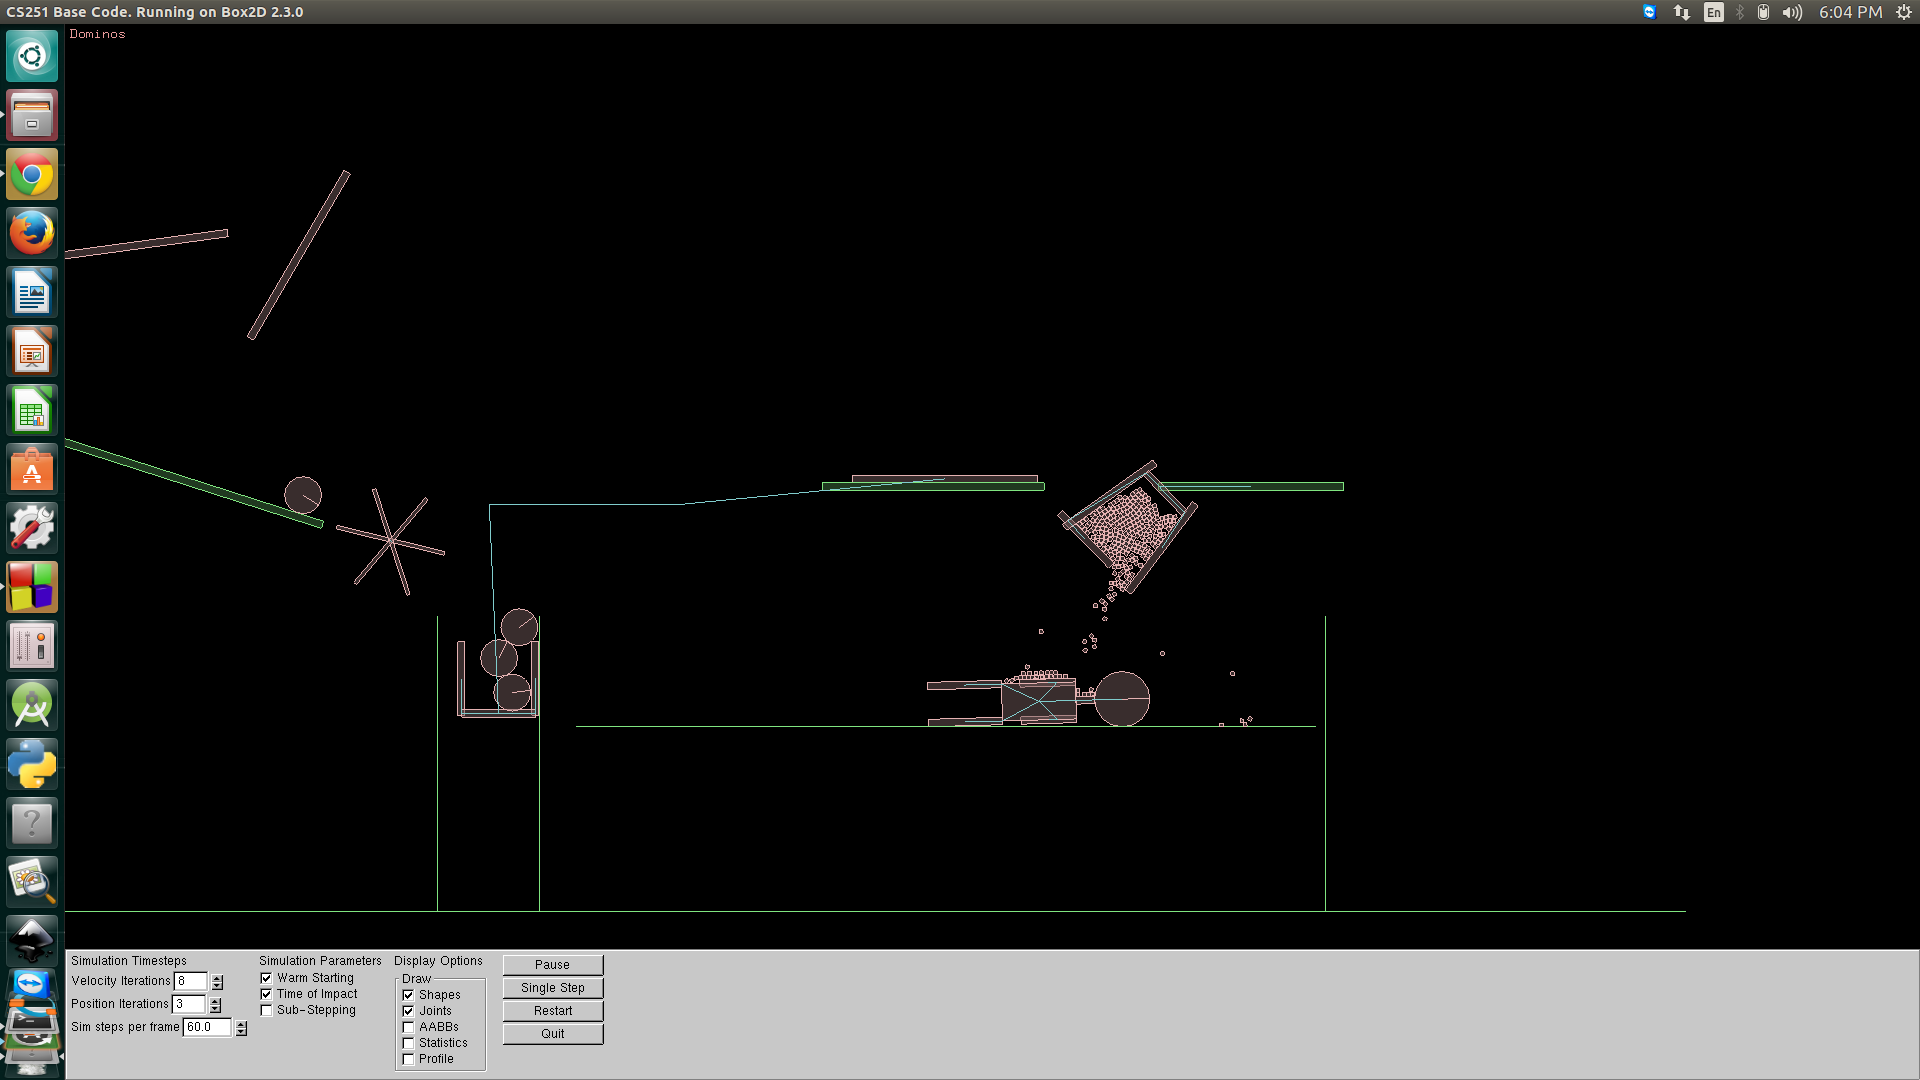
\includegraphics[scale=0.2]{project/images/bucket.png}
  \caption{\textbf{SECOND PULLEY}}
\end{figure}


\section{Bucket full of water}
\paragraph{
the construction of the bucket is similar to the oopen box.
just that the angles of the side blocks are changed.
also it has a lid which is also a block attached using a weld joint.
the water is made using small blocks of size 0.1/0.1
The bucket is attached to a static rectangular plank on the right side, with a revolute joint.
It is also supported using the plank which is connected to the pulley.
now when the pulley was disturbed the plank moves left and hence the bucket looses balance and rotates around the revolute joint.
now the water from the bucket falls down due to gravity on the face of the man and the man wakes up.
}
\begin{figure}[H]
  \centering
    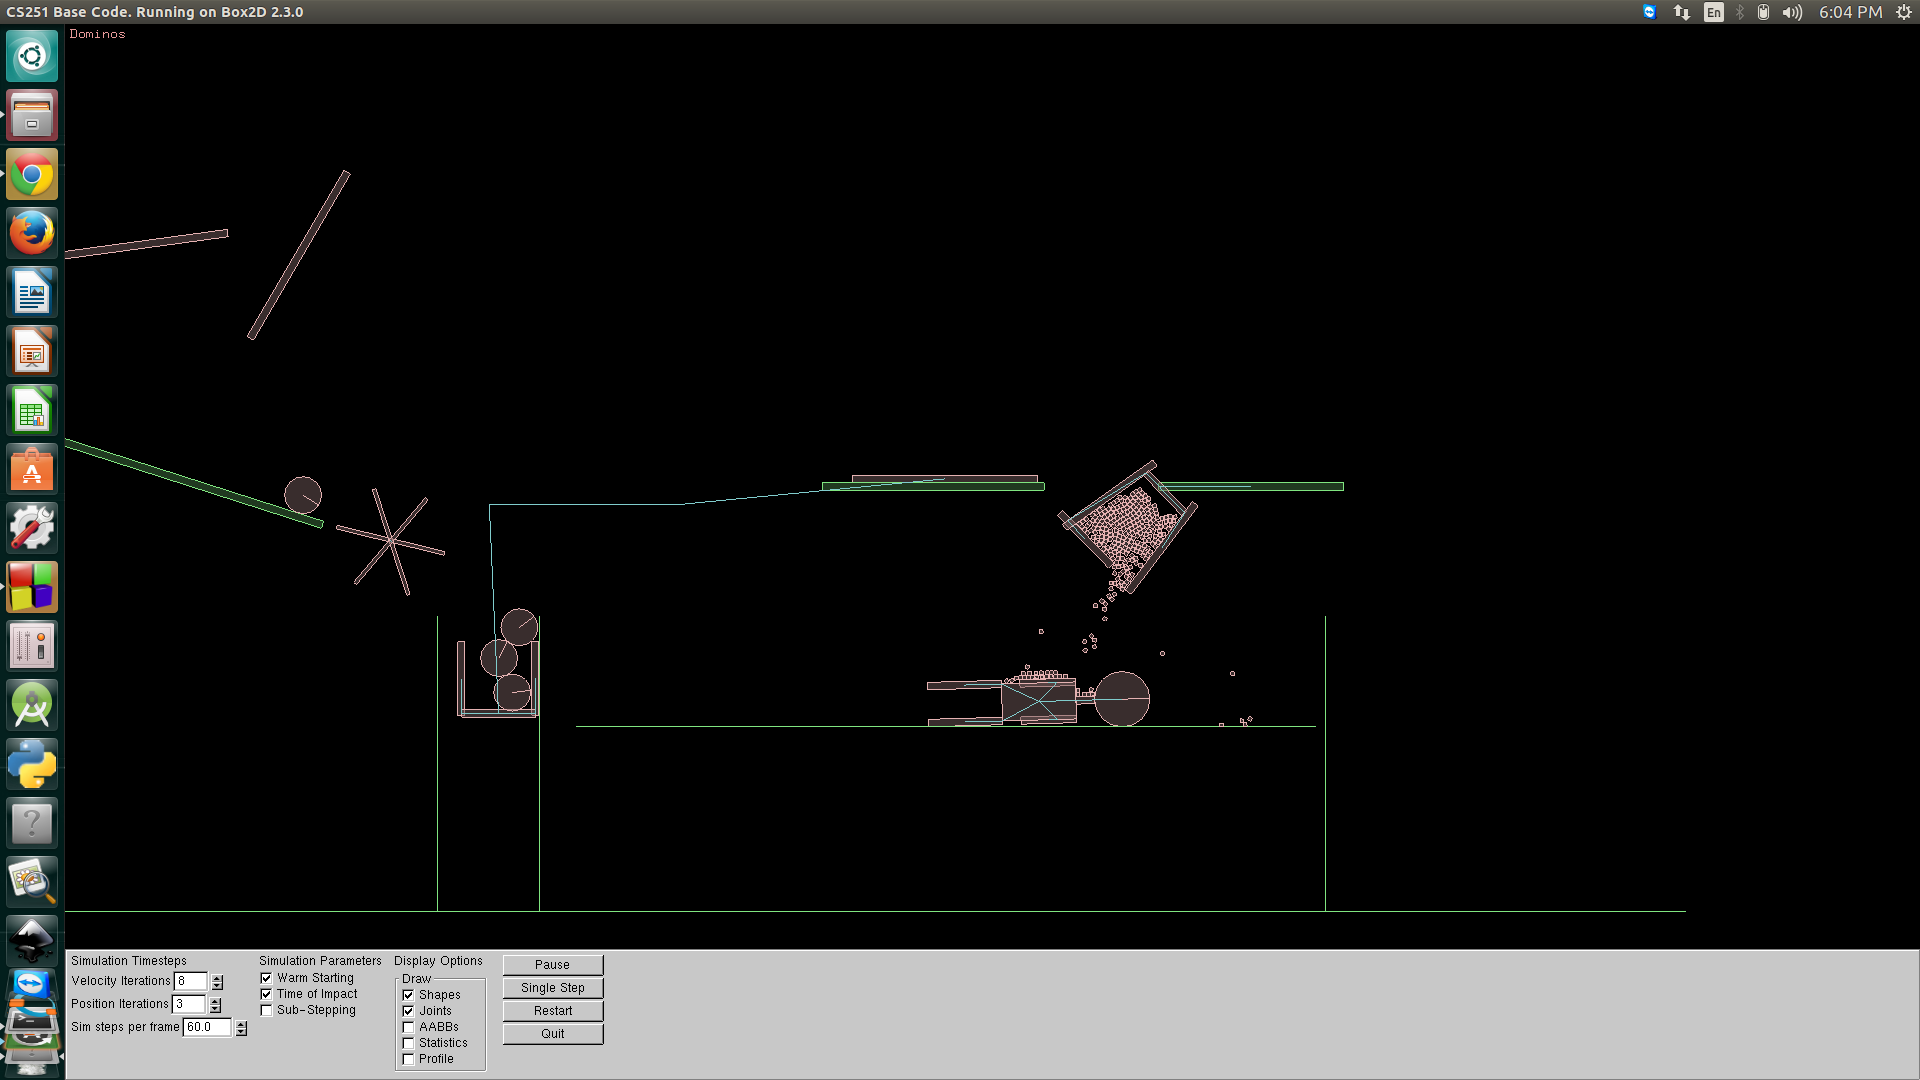
\includegraphics[scale=0.2]{project/images/bucket.png}
  \caption{\textbf{BUCKET}}
\end{figure}

 % adds the Project Design
\chapter{Contributions}


We distributed the work among us and did our individual parts and then combined it to get the final output. 
 Here are some of the works we did:
 \section{Divakar Reddy Naru}
 1) Documented the code using Doxygen \\
2) Created the major parts of the simulation which trigger various contraption for the project \\
3) Maintained the Project report using LateX \\
4) Created the slides for project review using beamer 
 \section{ Vishal Babu Bhavani} 
1) Designed the simulation. \\
2) Created the Newton's Pendulum Class, Pipe Class, Floating Balloon Class \\
3) Synchronised the simulation \\
4) Designed webpage for the Project \\
5) Wrote Makefile 
 \section{Pushyarag Yadagiri} 
1) Implemented different custom objects like motor, revolution launcher, custom pulley, bucket with water, clock etc \\
2) Helped team mates to maintain Git Repo with appropriate Version control \\
3) Created Video demo of the simulation \\
4) Worked for the makefile and profiling of data \\


%\input{project/system-design.tex}
\chapter{Simulation Testing}
\section{Bucket of water}

\begin{figure}[H]
  \centering
    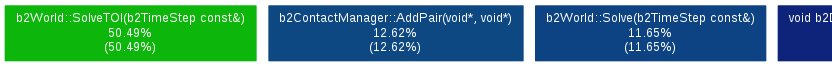
\includegraphics[scale=0.4]{project/images/infi_water.png}
  \caption{\textbf{call graph for water of very small size}}
\end{figure}

\paragraph{
The above is the call graph when we tried to implement bucket and water.
we made the size of water articles very small and made  the number of particles very large ,because of which the solveTOI function took very large time .we resolved it by increasing the size and reducing the number of particles.
the final call graph is as below.
}

\begin{figure}[H]
  \centering
    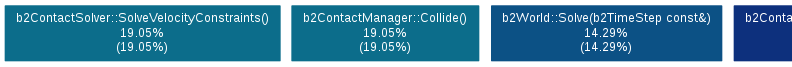
\includegraphics[scale=0.4]{project/images/normal_water.png}
  \caption{\textbf{call graph for final bucker and water}}
\end{figure}



We also generated and analysed the call graphs of various complex objects(those created using simple objects like blocks,spheres,etc) like cloeck,sesaw etc and didnot find any important optimisations to be made.


\section{Clock}

\begin{figure}[H]
  \centering
    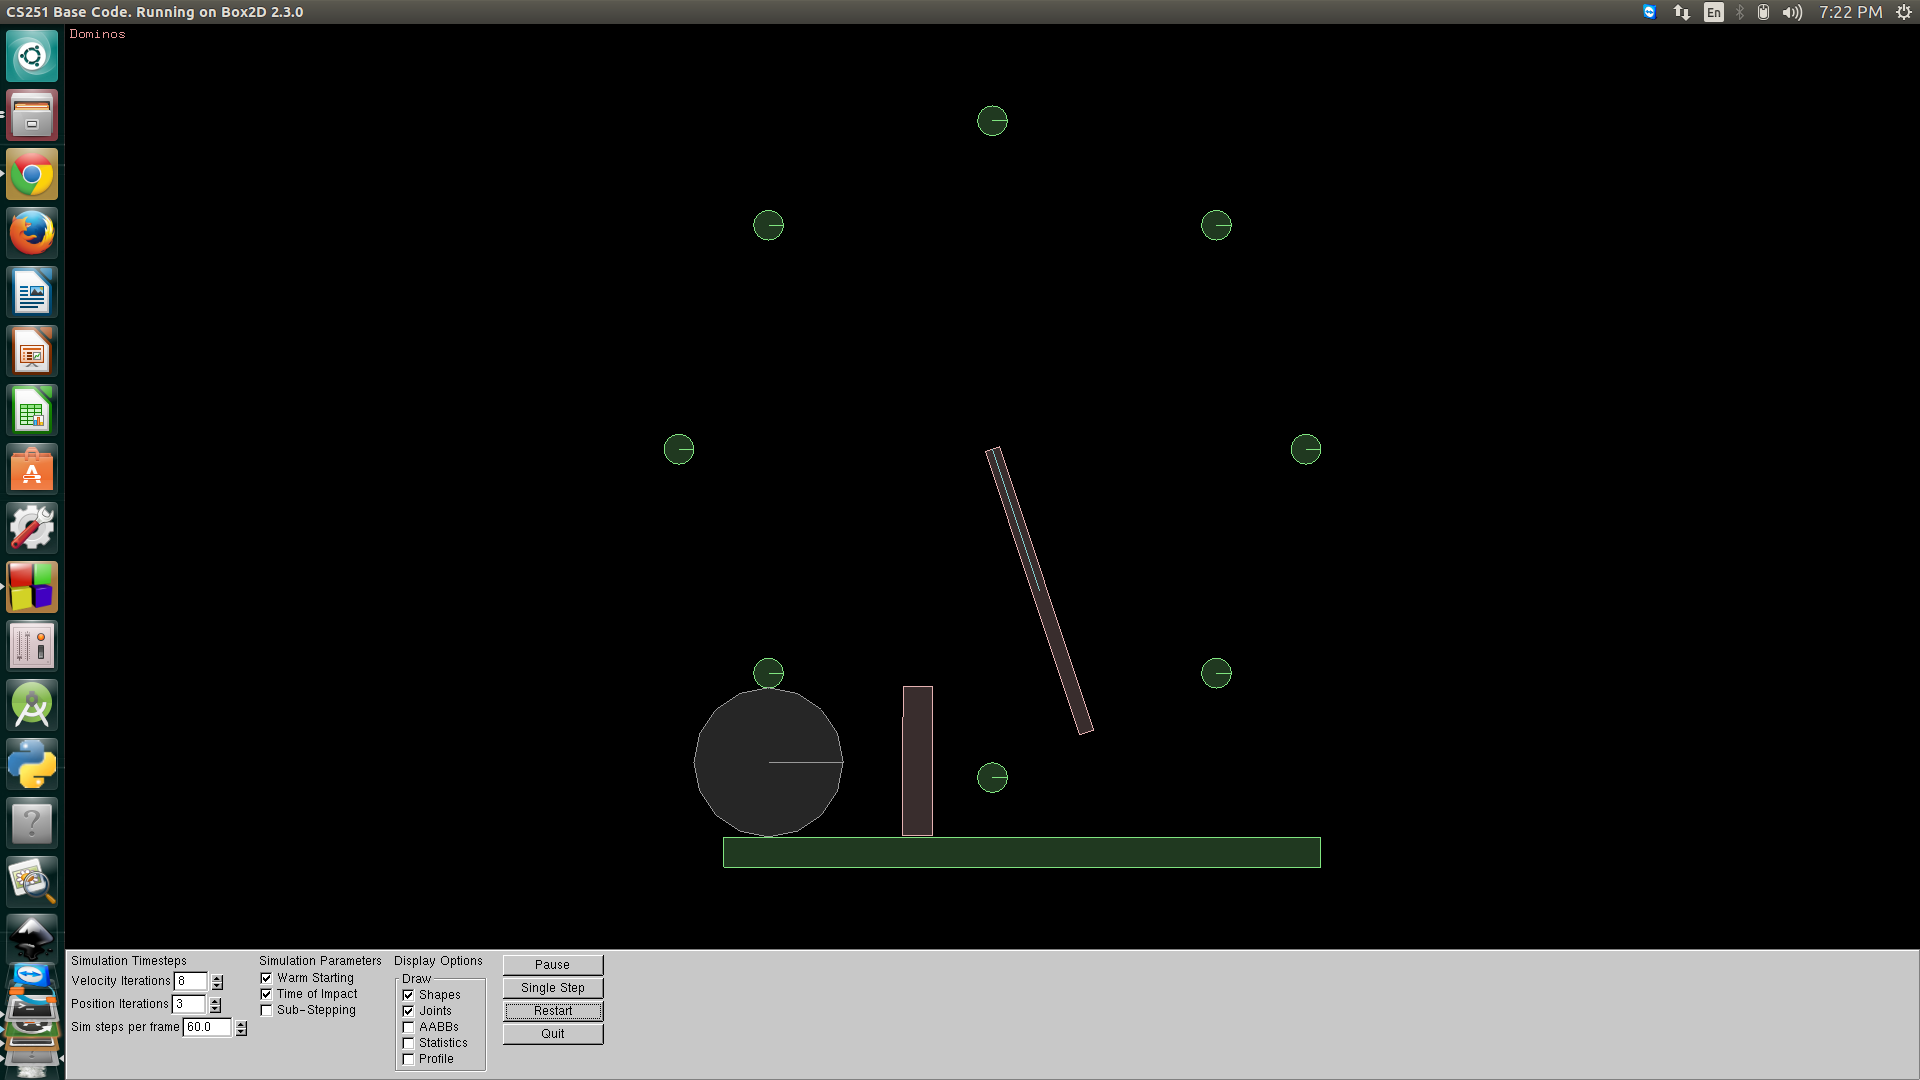
\includegraphics[scale=0.4]{project/images/clock.png}
  \caption{\textbf{call graph for clock}}
\end{figure}

\section{Seesaw and pulley}

\begin{figure}[H]
  \centering
    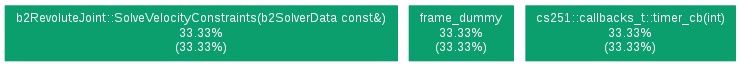
\includegraphics[scale=0.4]{project/images/seesaw.png}
  \caption{\textbf{call graph for seesaw and pulley}}
\end{figure}

\section{Curves and newton's pendulum}

\begin{figure}[H]
  \centering
    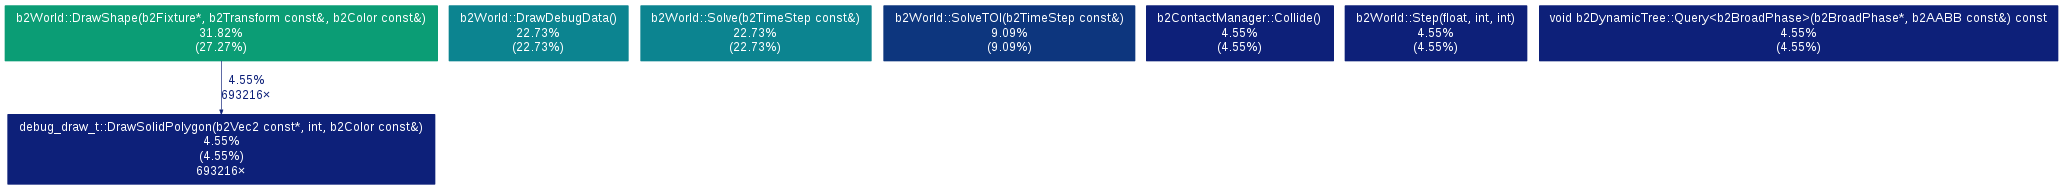
\includegraphics[scale=0.4]{project/images/curves.png}
  \caption{\textbf{call graph for curves and newton's pendulum}}
\end{figure}
%\chapter{Project Planning}
\section{Frequency estimation of a periodic wave}
\paragraph{}
We started by calculating the frequency estimation of a periodic wave.The technique did not require us to use Fourier transform so it made things simple.Our approach to this was the rule that frequency of a peridoc signal is proportional to the number of maxima or minima in a fixed finite time interval.
\section{Frequency estimation of a non-periodic wave}
\paragraph{}
After we were successful in finding the period of a periodic wave,the next challenge was that the audio signals practically are not exactly periodic because of the minute disturbances in the medium which cause considerable fluctuations in the audio signal in the order of period.So we changed the approach and calculated the period by brute-force method i.e varying period within certain limits and checking which value of period satisfied the required conditions the most.
\section{Frequency estimation with Fourier Analysis}
\subsection{No Harmonics}
\paragraph{}
The above method was successful but it was slow,then we finally resorted to using the fast Fourier transform provided by MATLAB,our operating environment.But even that was not enough because if T is the period then nT, where n=2,3,4...... can also be the period.So we were not sure if we got the right frequency.So we created an artificial sine wave with the detected frequency and compared with the input.As doubted errors occurred due to above reason.
\subsection{In presence of Harmonics}
\paragraph{}
Fortunately,the solution to the above problem was the problem itself.If more than one harmonics are present then we can find the fundamental frequency by two methods i.e by finding the least frequency in them or by calculating the difference between two consecutive harmonics.In almost all the cases both give the same result.But in few cases the first methods fails if the least frequency is undetected.If something like that happens the second method ensures the correctness of the frequency.
\section{Note Detection}
\paragraph{}
Once we were able to calculate the frequency of a note the next challenge was to isolate the note from the audio input.Since our code works only if the input contains a single note and no other signals.Initially we limited the domain of the input and designed a note detection method which works on the fact that a note begins with fast increase in intensity and ends with decrease in intensity below a threshold.The method worked perfectly except when a two notes were very close i.e when a note started before a note ended.So two notes were taken as a single note and thereby resulted in errors while detected frequency in that region.Since the note detection was not the main agenda of our project we learned from external sources to develop the note detection which used Gaussian filters and other advanced functions provided by MATLAB.



\chapter{Screenshots of Project}
\vspace{2cm}
\begin{figure}[H]
  \centering
    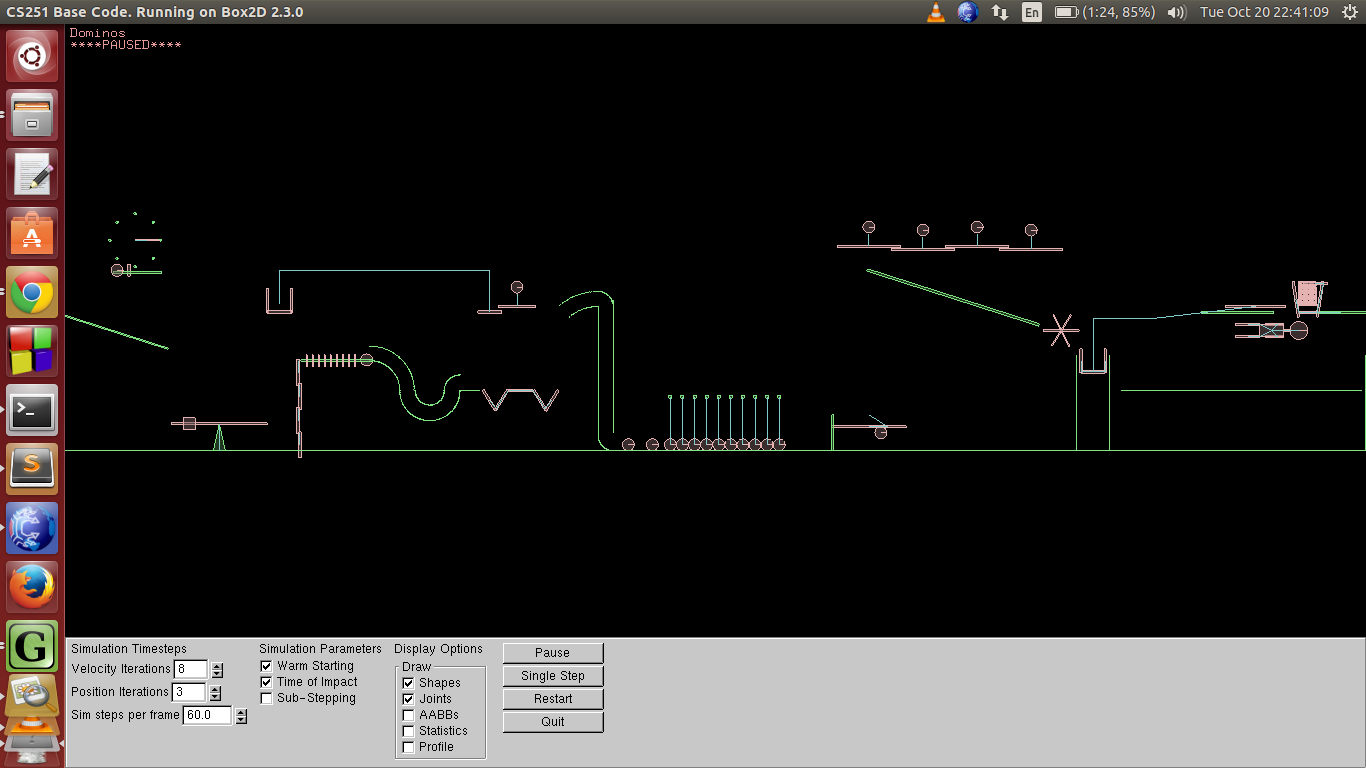
\includegraphics[scale=0.2]{project/images/screenshot.png}
  \caption{\textbf{screenshot 1}}
\end{figure}
\begin{figure}[H]
  \centering
    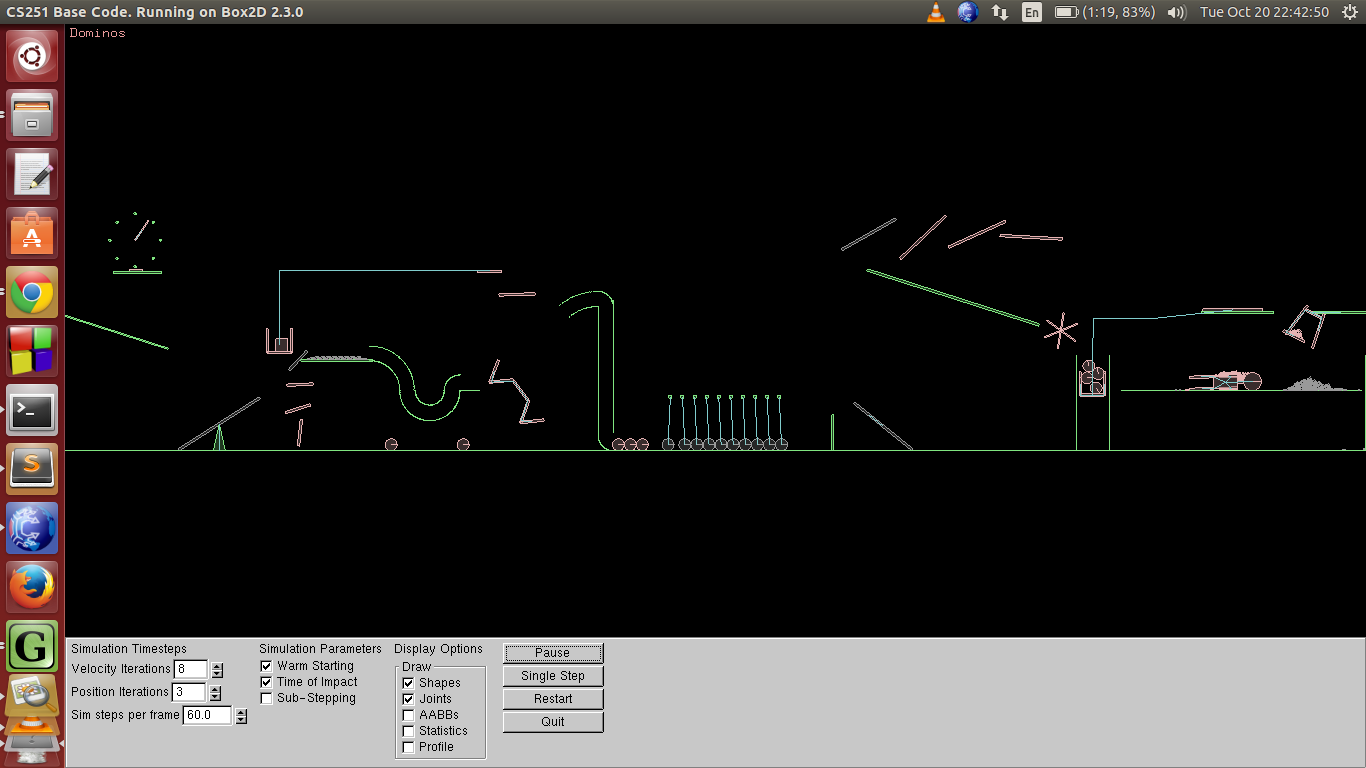
\includegraphics[scale=0.2]{project/images/screen.png}
  \caption{\textbf{screenshot 2}}
\end{figure}

%\chapter{Requirement Analysis}
\section{INPUT AUDIO FEATURES}
\paragraph{} The program uses auto note detection which operates based on the variations in the intensity of sound. In almost all the cases there is an sudden increase in the intensity i.e proportional to the square of the values in the input array.Thus for efficient note detection the input audio signal must have considerable amount of variation when a note begins.This can be assured when the sound intensity of noise in the signal is considerably less than the note sound intensity.
\begin{figure}[H]
 \centering
   \includegraphics[height= 7.5cm, width=15cm]{project/images/MAIN.png}
  \caption{\textbf{Difference in noise and note }}
  
\end{figure}
\paragraph{} The manual tuning requires the user to set a threshold above which the note can be detected.This feature allows him to choose only the required regions to find frequency.It checks if the intensity is greater than the given threshold and plots the graph.The points thus recognised are stored in an array for processing.
%\input{project/conclusion.tex} % adds the Scheduling and Planning page
\addcontentsline{toc}{chapter}{References}

\medskip
 
\bibliographystyle{unsrt}
\bibliography{ref}
 % adds the References page

\end{document}